\documentclass[11pt]{article}
\usepackage[margin=1in]{geometry}
\usepackage{amsmath,amssymb,amsthm}
\usepackage{graphicx}
\usepackage[hidelinks]{hyperref}

\newcommand{\arxiv}[1]{\href{https://arxiv.org/abs/#1}{arXiv:#1}}
\newcommand{\R}{\mathcal R}

\title{Literature-Implied Answer: Positive UMD-Lattice Semigroups Need Not Be \(\R\)-Sectorial}
\author{FA/Banach run \texttt{fa\_banach\_001}}
\date{2026-06-14}

\begin{document}
\maketitle

\section*{Status}

This packet records a \emph{literature-implied} negative answer to the
positivity-only UMD-Banach-lattice version suggested by the open-problem
cluster in Fackler's survey \arxiv{1407.1142}.  It is not claimed as a new
counterexample and it is not an answer to the contractive variants.

The source problem cluster asks whether positivity and/or contractivity of the
semigroup generated by \(-A\) force bounded \(H^\infty\)-calculus, bounded
imaginary powers, or \(\R\)-analyticity.

\begin{center}
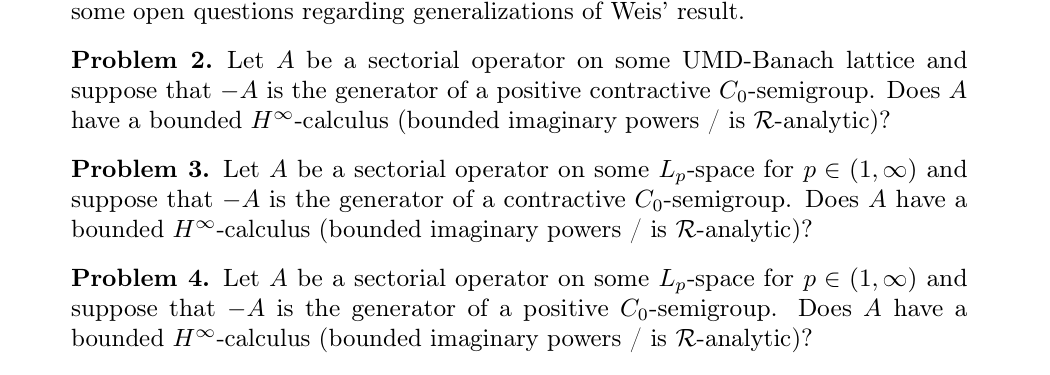
\includegraphics[width=0.96\linewidth]{figures/source_open_problems_crop.png}
\end{center}

\section*{Supporting Literature}

Fackler's later paper \arxiv{1411.4240} proves the following theorem.

\begin{center}
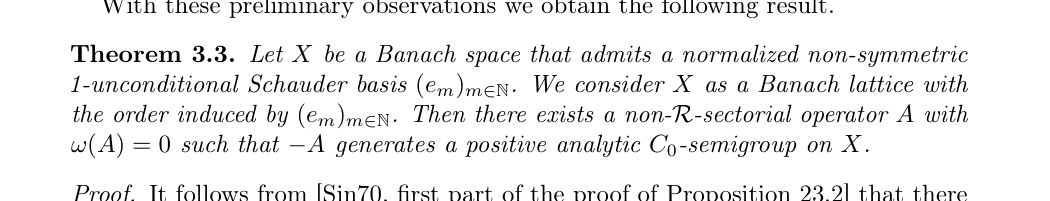
\includegraphics[width=0.96\linewidth]{figures/supporting_theorem_3_3_crop.png}
\end{center}

The same paper immediately specializes the theorem to the UMD Banach lattices
\(\ell_p(\ell_q)\), \(p,q\in(1,\infty)\), \(p\ne q\).

\begin{center}
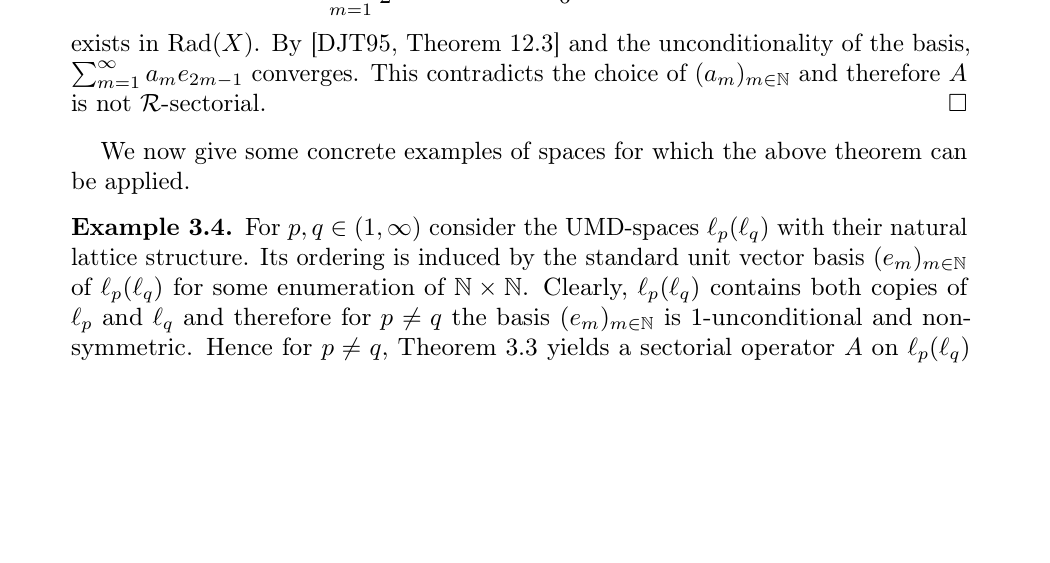
\includegraphics[width=0.96\linewidth]{figures/supporting_example_3_4_crop.png}
\end{center}

\begin{center}
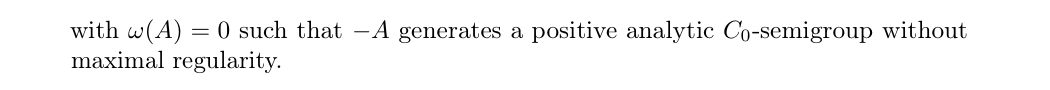
\includegraphics[width=0.96\linewidth]{figures/supporting_example_3_4_continuation_crop.png}
\end{center}

\section*{Implication}

Choose \(p,q\in(1,\infty)\) with \(p\ne q\).  The space
\(\ell_p(\ell_q)\), with its natural lattice structure, is a UMD Banach
lattice.  By Theorem 3.3 and Example 3.4 of \arxiv{1411.4240}, there exists a
sectorial operator \(A\) on \(\ell_p(\ell_q)\) such that
\[
  \omega(A)=0,
  \qquad
  -A \text{ generates a positive analytic } C_0\text{-semigroup},
\]
but \(A\) is not \(\R\)-sectorial.

The survey \arxiv{1407.1142} recalls the implication chain relevant here:
bounded \(H^\infty\)-calculus implies bounded imaginary powers, and on UMD
spaces bounded imaginary powers imply \(\R\)-sectoriality.  Therefore the above
operator \(A\) cannot have bounded imaginary powers and cannot have a bounded
\(H^\infty\)-calculus.  Since it is not \(\R\)-sectorial, it is also not
\(\R\)-analytic in the sense of the source problem cluster.

Thus positivity alone on UMD Banach lattices does not force the regularity
properties asked for in the cluster.

\section*{Limitations}

\begin{itemize}
\item The semigroup in \arxiv{1411.4240} is positive analytic, but no
  contractivity is asserted.  Hence this packet does not settle the positive
  contractive UMD-Banach-lattice problem in \arxiv{1407.1142}.
\item The counterexample space \(\ell_p(\ell_q)\), \(p\ne q\), is a UMD
  Banach lattice but not a classical scalar \(L_p\) space.  Hence this packet
  does not settle the positive \(L_p\) problem or the contractive \(L_p\)
  Matsaev problem.
\item The packet records a direct literature implication from Fackler's later
  theorem; it does not add a new construction beyond that theorem.
\end{itemize}

\end{document}
